\begin{table}[h!]
	\caption{The KNeighborsClassifier parameters}
	\begin{tabular}{ | l | l | p{7cm} |}
		\hline
		\textbf{Parameter} & \textbf{Default} & \textbf{Description}\\
		\hline
		$n\_neighbors$ & 5 & Number of neighbors to use.\\
		\hline
		$weights$ & uniform & weight function used in prediction.
		
		‘uniform’ : All points in each neighborhood are weighted equally. 
		
		‘distance’ : weight points by the inverse of their distance.\\
		\hline
		$algorithm$ & auto & Algorithm used to compute the nearest neighbors: ball\_tree, kd\_tree, brute (brute-force search) or auto. The last will attempt to decide the most appropriate algorithm based on the values passed to fit method.\\
		\hline
		$metric$ & minkowski & the distance metric to use for the tree.\\
		\hline
		$p$ & 2 & Power parameter for the Minkowski metric. When p = 1, this is equivalent to using manhattan\_distance, and euclidean\_distance for p = 2.\\
		\hline
	\end{tabular}
	\label{table:KNNdefaults}
\end{table}
The following set of hyper-parameter values was used:
\begin{itemize}
	\item n\_neighbors: [2, 3, 5, 7, 10, 15, 20]
	\item weights: ['uniform', 'distance']
	\item algorithm: ['ball\_tree', 'kd\_tree', 'brute']
	\item metric: ['minkowski']
	\item p: [1, 2, 3, 4, 5]
\end{itemize}
\subsubsection{Results}
\begin{table}[h!]
	\caption{Grid search output}
	\centering
	\begin{tabular}{ | l | c | c | c | c | c | c |}
		\hline
		$\bf{params_n}$ & \bf{n\_neighbors} & \bf{weights} & \bf{algorithm} & \bf{metric} & \bfseries{p}\  & \bfseries{log\_loss} \\ \hline
		$params_1$ & 20 & 'uniform' & 'brute' & 'minkowski' & 3 & 0.9871  \\ \hline
		$params_2$ & 20 & 'uniform' & 'kd\_tree' & 'minkowski' & 3 & 1.0305 \\ \hline
		$params_3$ & 15 & 'distance' & 'ball\_tree' & 'minkowski' & 3 & 1.0478 \\ \hline
		$params_4$ & 20 & 'uniform' & 'ball\_tree' & 'minkowski' & 5 & 1.1013 \\ \hline
		$params_5$ & 15 & 'distance' & 'ball\_tree' & 'minkowski' & 5 & 1.1176 \\ \hline
	\end{tabular}
\end{table}
%\vspace{2mm}
\begin{figure}[h!]
	\centering
	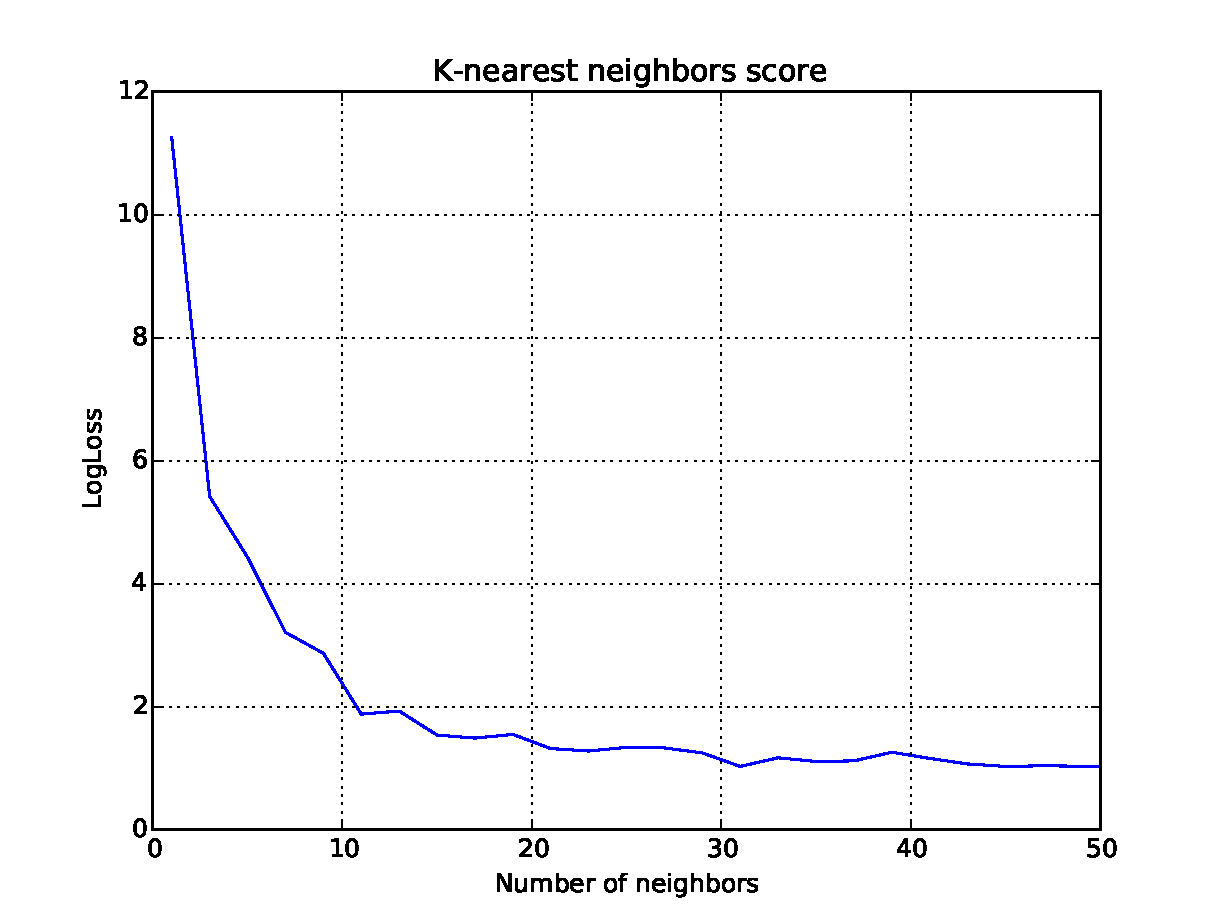
\includegraphics[width=0.8\textwidth]{KNN_scores}
	\caption{Scores varying the number of neighbors}
	\label{fig:KNN_scores}
\end{figure}
Figure \ref{fig:KNN_scores} was plotted by setting the $params_1$ obtained from the grid search and varying the number of neighbors. It can be appreciated that the LogLoss stops improving significantly passed the 30th neighbor.\\
\begin{figure}[h!]
	\centering
	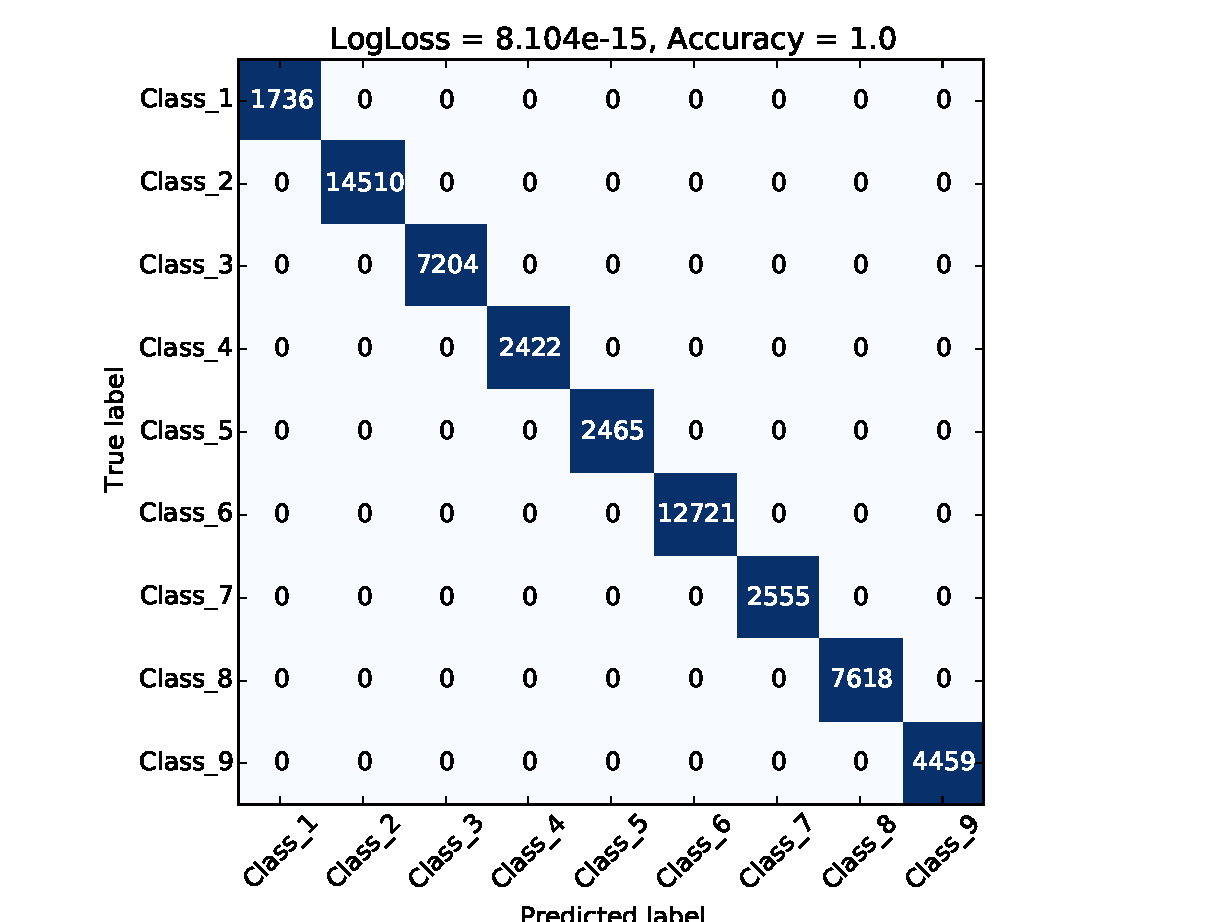
\includegraphics[width=0.7\textwidth]{KNNcm_train}
	\caption{k-NN confusion matrix using training dataset}
	\label{fig:KNNcm_train}
\end{figure}
\begin{figure}[h!]
	\centering
	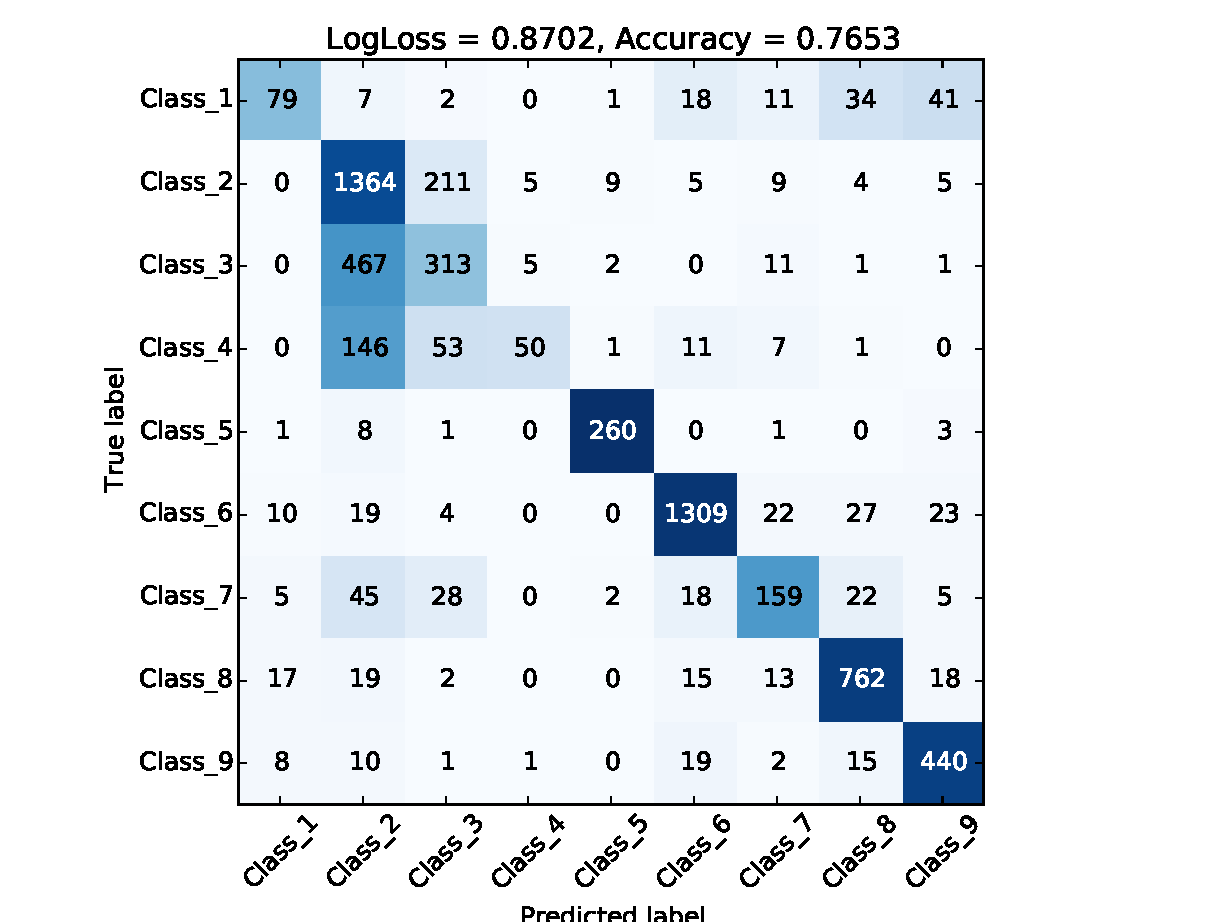
\includegraphics[width=0.7\textwidth]{KNNcm_test}
	\caption{k-NN confusion matrix using testing dataset}
	\label{fig:KNNcm_test}
\end{figure}\\
Because of the nature of the algorithm, measuring performance over the training set will always output a perfect accuracy because the points evaluated are exactly the same. The confusion matrix using the testing set gives us interesting results and an insight on how the data is arranged despite it's high dimensionality. There are lots of neighboring points between class 2, 3, and 4 which makes them the hardest classes to classify.\\